
\section{Results}

We generate the visibility graph for each sub-region of interest using the time-magnitude sequences shown in Fig.~\ref{fig:mag-time}. The number of nodes in each graph is the same as the (declustered) number of events shown in Table \ref{tab:seismicity}, and the links between inter-visible events are established following the condition in equation (\ref{eq:vg}), as in the example shown in Fig.~\ref{fig:vg}. (We do not include a visualization of the complete sequence graphs because the links are so many, it is only practical to visualize the graphs of short sequences.) We then collect information about the number of inter-visibility links associated with each event (connectivity degree, $k$) and categorize the events in magnitude bins of size $\Delta M = 0.1$, as mentioned in the Methodology section. Figure \ref{fig:km} shows the scattered distribution of events in the magnitude-connectivity degree plane for each sub-region. The figure shows that, in general, the value of $k$ increases with $M_w$. Figure \ref{fig:km} also shows the results of obtaining linear $k$-$M$ regressions for each dataset and the values of the $k$-$M$ slopes for the three seismic zones.

\begin{figure*}[t]
	\centering
	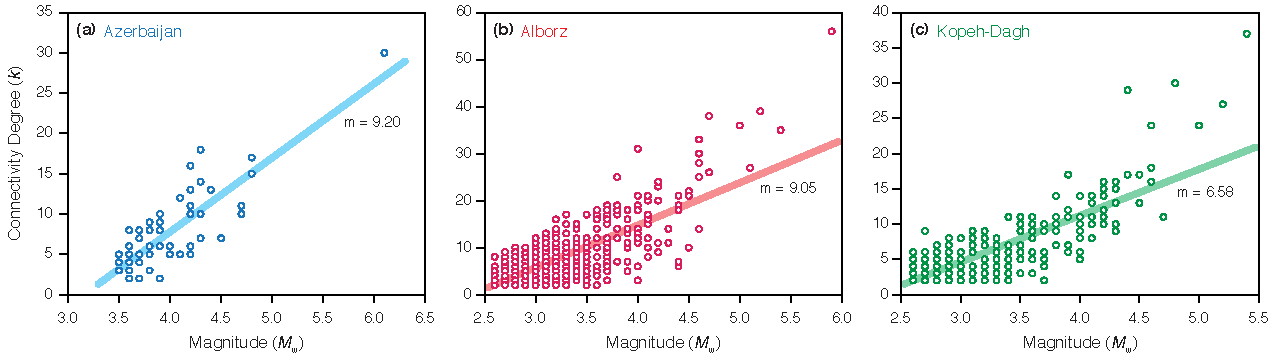
\includegraphics[width=\textwidth]{figures/pdf/figure-06} 
	\caption{Scattered distribution of events in the magnitude-connectivity degree plane and linear regressions obtained for the $k$-$M$ relationships for the three seismic regions in northern Iran. The value next to each of regression line corresponds to the slope of the line, which is referred here as the $k$-$M$ slope. The color version of this figure is available only in the electronic edition.}
	\label{fig:km}
\end{figure*}

Next, we examine the relationship between the $b$-values from Table \ref{tab:seismicity} and the $k$-$M$ slope values shown in Fig.~\ref{fig:km}. Figure \ref{fig:regression} shows the scattered results for $k$-$M$ slope versus $b$-value for the three tectonic seismic regions in northern Iran along with the data-points obtained for the analysis of the magnitude-time sequences of the Mexican subduction zone \citep{Telesca2013} and the Pannoninan seismic zone \citep{Telesca2014}, as well as other experimental results \citep{Telesca2014-pone}. Figure \ref{fig:regression} also includes the results of different linear regressions between the $b$-value and the $k$-$M$ slope. Each regression reflects the addition of new data-points from different studies. Note that the regression improves as new data-points are added, which is indicated by the correlation coefficient $R$, also included in the figure. The correlation fitting various regional seismic data was previously pointed out by \citet{Telesca2014}.

According to these results, a universal relationship between the $b$-value and the $k$-$M$ slope ($m$) can be expressed as:
% 
\begin{equation}
	b = 0.078 + 0.085 m \, .
	\label{eq:universal.bm}
\end{equation}

\begin{figure}[h]%[t]
	\centering
	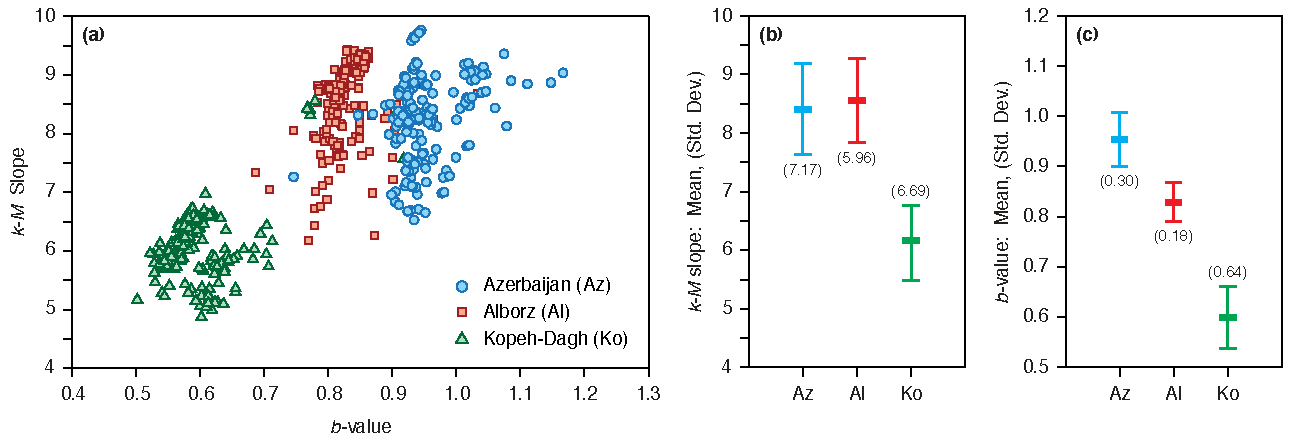
\includegraphics[width=0.45\textwidth]{figures/pdf/figure-07} 
	\caption{Correlation between $k$-$M$ slope and $b$-value as drawn from the results of the present study for the region of northern Iranian and three other previous studies, including analysis of the Mexican subduction zone \citep{Telesca2013}, the Pannonian seismic zone \citep{Telesca2014}, and results from two experiments \citep{Telesca2014-pone}. The lines represent linear regressions obtained to fit the different data points, considering different combinations. The values of the correlation coefficient, $R$, are indicated for each regression line. The color version of this figure is available only in the electronic edition.}
	\label{fig:regression}
\end{figure}

Another aspect of interest is the stability of the data points themselves. Note that as presented in Fig.~\ref{fig:regression}, the analysis of the sequences shown in Fig.~\ref{fig:mag-time} only contribute one data point per region of interest. Furthermore, each data-point comes from sequences that vary significantly in terms of the number of events and seismic parameters (see Table \ref{tab:seismicity}). 

\citet{Telesca2013} observed that the value of the $k$-$M$ slope is not particularly sensitive to the sample size in the sequence---at least not when considering sufficiently large sequences. On the other hand, as we will see below, if the sequence window is sufficiently small, then the $k$-$M$ slope value shows a relative dependence on time and thus provides insight about the variation of the seismicity as the sequence progresses. Note also that the threshold value of $M_c$ is significantly smaller for Azerbaijan than for Alborz or Kopeh Dagh. This is due in part to the fact that the latter two zones were more seismically active in the time period under consideration. However, according to \citet{Telesca2012}, the threshold magnitude has a minor effect in the graph parameters.

To further explore the sensitivity of the graph properties to the number of events in each catalog and the value of the minimum magnitude, we randomly picked a significant number of sub-sequences from within the initial catalog compiled for each region, and repeated the analysis for each sub-sequence. In total, for each region, we extracted 200 new sub-sequences from the initial (pre-declustering) catalog. The number of events in each sub-sequence was varied randomly but chosen to be large enough to represent the seismic characteristics of each region. In particular, the minimum size of each sub-sequence was set to be $n \geq 150$, and the maximum size in the sequence was set to be as large as the original catalog (pre-declustering; see Table \ref{tab:seismicity}). We forced the random sub-sequences to progress positively in time without altering the natural occurrence of events. In other words, we randomly determined the initial event and the sub-sequence size (number of events to be considered), and then picked that number of events following the initial earthquake in the sub-sequence. Next, we determined the value of $M_c$ and $b$ as previously done for the complete catalogs, created the graph for all events with $M \geq M_c$, and extracted the connectivity degree of the events in each sub-sequence. 

\begin{figure*}%[t]
	\centering
	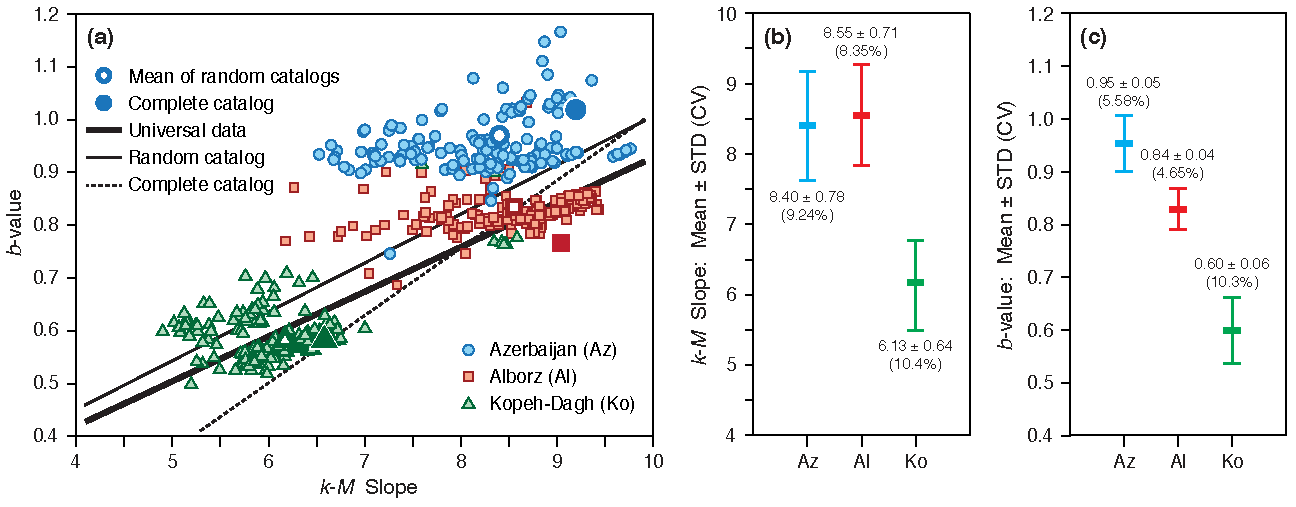
\includegraphics[width=0.9\textwidth]{figures/pdf/figure-08} 
	\caption{\textbf{(a)} Correlation between $k$-$M$ slope and $b$-values for 200 random sequences extracted from the initial catalogs of the three northern Iranian seismic regions considered in this study (scattered symbols), including the mean values (empty symbols with thick border) and the data points obtained from the analysis of the complete catalog (solid symbols), along with the linear regressions of each sample as indicated in the legend. \textbf{(b)} Mean, $\pm1$ standard deviation, and coefficient of variation (in percent) for the $k$-$M$ slope values of the three seismic zones in northern Iran. \textbf{(c)} Same as part (b), but corresponding to the $b$-value. The color version of this figure is available only in the electronic edition.}
	\label{fig:random}
\end{figure*}

Figure \ref{fig:random}a shows scattered points for all the individual $k$-$M$ slope and $b$-value pairs for all the sub-sequences that were randomly picked from the initial catalogs of each region in northern Iran (small symbols). Figures \ref{fig:random}b and \ref{fig:random}c show the variability of the $k$-$M$ slope and $b$-value, respectively. These latter figures show the mean values of each parameter for all the random sub-sequences and the amplitudes of $\pm 1$ standard deviation, as well as the coefficients of variation (in percentage). Figure \ref{fig:random}a also includes the data points corresponding to the complete catalogs (large solid symbols); the points corresponding to the mean values of the $k$-$M$ slope and $b$, from Figs.~\ref{fig:random}b and \ref{fig:random}c (large hollow symbols); and the universal linear regression from equation (\ref{eq:universal.bm}) (thick line), as well as the linear regressions for northern Iran when using the complete catalogs (dashed thin line) and the random sub-catalogs (continuous thin line). 

The comparison between the mean values of the random sequences analysis versus the complete catalogs presented in Fig.~\ref{fig:random} indicates that there exists only a small bias, which is well within the standard deviation of the different value samples. We note that the values of the $k$-$M$ slope are slightly smaller when obtained with the random sequence analysis, whereas the $b$ values seem more stable. The comparisons of the regressions, however, indicate that the analysis of the random sub-catalogs leads to a result more in line with the universal results obtained when considering multiple seismic zones. The linear regression of the random sub-catalogs yields the following equation:
% 
\begin{equation}
	b = 0.080 + 0.093 m \, .
	\label{eq:iran.bm}
\end{equation}

Note that equations (\ref{eq:universal.bm}) and (\ref{eq:iran.bm}) have similar intercepts with the $b$-value axis, and only slightly different slope constants. In this particular case, the analysis for northern Iran leads to a relationship in which the $b$-value increases more rapidly with $m$ than in the case of the regression obtained for the universal data. The similarity between the two equations, however, is a positive sign of the stability of the method.

\begin{figure*}%[t]
	\centering
	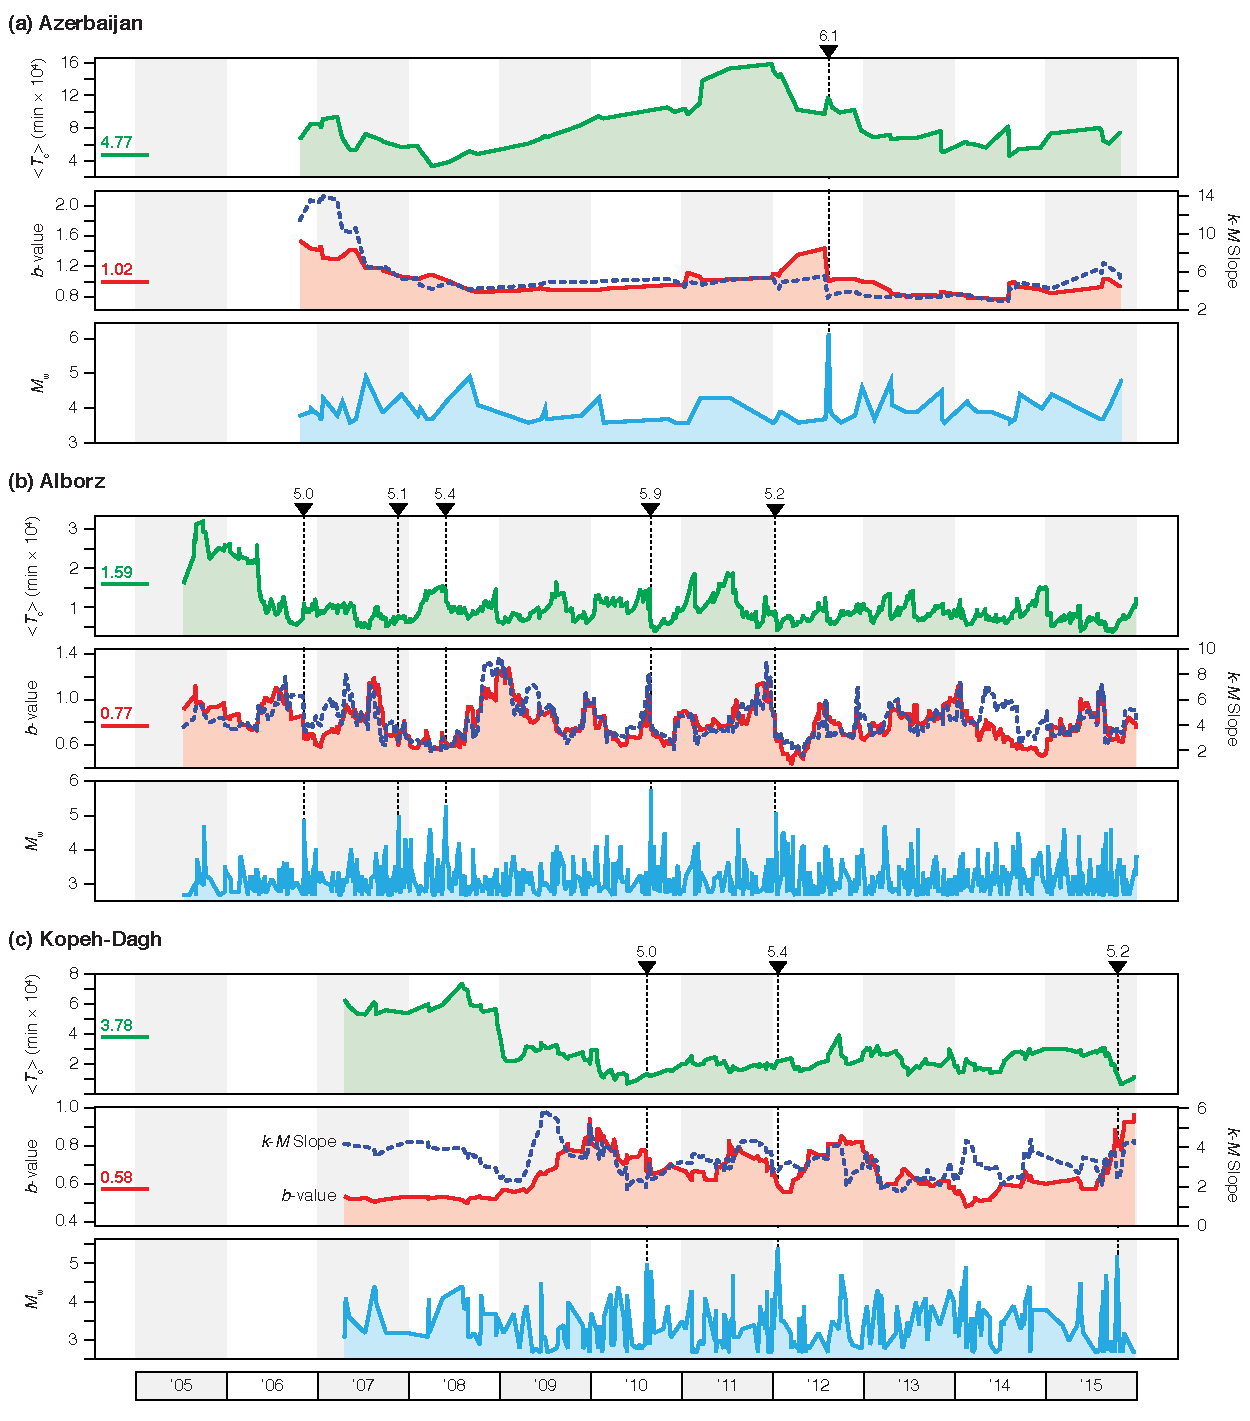
\includegraphics[width=\textwidth]{figures/pdf/figure-09} 
	\caption{Variation of <$T_c$>, $k$-$M$ slope and $b$-value as with respect to time for three seismic zones for a moving window analysis of the visibility graphs of sub-sequences of 20 consecutive events, along with the magnitude of events in the 2005--2015 period. Black triangles indicate the occurrence of major earthquakes in each of the regions, with the corresponding magnitude at the top of each symbol. In the middle frame of each region, the dashed line corresponds to the $k$-$M$ values, whereas the continuous plot shows the variation of the $b$-value. The color version of this figure is available only in the electronic edition.}
	\label{fig:tc}
\end{figure*}

We now investigate the relationship of the parameters obtained through the visibility graph analysis with time. Here, the visibility graph analysis is done by windows of equal number of events moving in time across the catalog sequence. The number of events in the window is kept fixed independently of the time between them, and the results are associated with the last event in the window. In this case, we are interested in using a small number of events to capture the relevance of each new event as the window moves in time. We tried different numbers and finally chose 20 events as the moving window sequence size. This selection was also convenient given the smaller total number of declustered events in the catalog of Azerbaijan. When we tested larger number of events, we found that we could not properly observe the changes in the different parameters with time. On the other hand, when we used smaller sequence sizes, the values deviated more significantly from the random and complete catalog results obtained previously. At this point it is also of interest to compute the value of <$T_c$> explained in the Methodology section.

Figure \ref{fig:tc} shows the variation of <$T_c$>, the $k$-$M$ slope, and the $b$-value with time for each of the three seismic zones in northern Iran. The time-magnitude sequence is also included for reference. Note that the behavior of the $k$-$M$ slope and the $b$-value is very similar along time for all three zones. This is consistent with the results presented before. We note that there seems to be a correlation between the behavior of the $b$-value in time with the occurrence of some of these larger events. In particular, some of the events in the figure seem to coincide with a drop in the $b$-value. 

The decline of the $b$-value before large earthquakes has been studied in other regions before \citep[e.g.,][]{Wyss2000, Wyss2006, Schorlemmer2005, Chan2012}. In the context of the visibility graph analysis, \citet{Telesca2016} observed a decrease in <$T_c$> before the large earthquake of the western India earthquake sequence. We recognize, however, that the lack of larger ($M>6$) events in our region of interest in the last decade prevents us from drawing a stronger conclusion on this regard. 
